\subsection*{BVP framework: The FEMSystem class}

\begin{frame}
  \begin{minipage}[h]{.45\textwidth}
    \begin{center}
      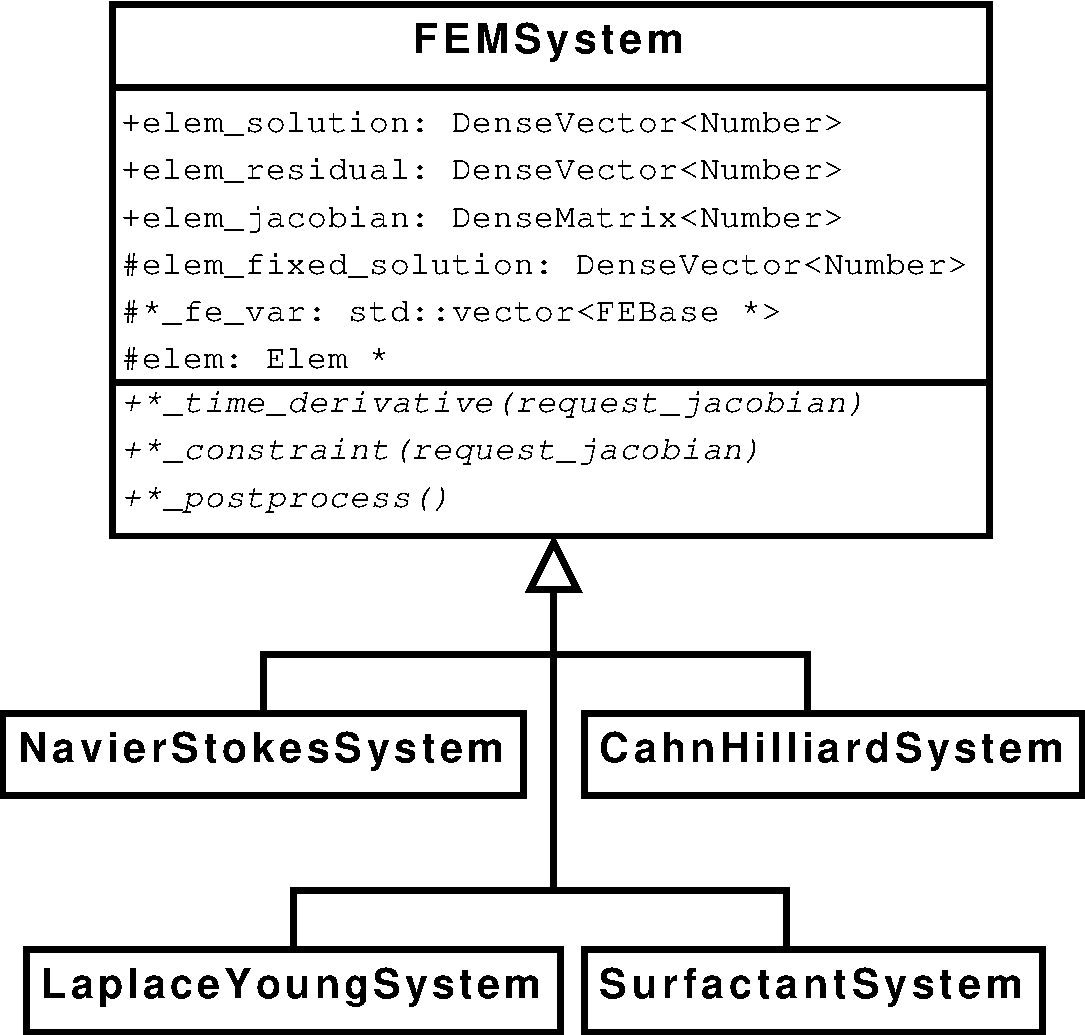
\includegraphics[width=.9\textwidth]{figures/FEMSystem}
    \end{center}
  \end{minipage}
  \begin{minipage}[h]{.5\textwidth}
      \begin{itemize}
      %\item Generalized IBVP representation
      %\item FEMSystem does all initialization, global assembly
      \item
        User provides (weak form) weighted residuals
        \begin{equation}
          \nonumber
        \left(M\frac{\partial u}{\partial t}, v_i \right) =
        \left(F\left(u\right), v_i\right)
          \end{equation}
        \item And/or constraints
        \begin{equation}
          \nonumber
          \left(G\left(u\right), v_i\right) = 0
        \end{equation}
      \end{itemize}
  \end{minipage}
\end{frame}
